%! Author = ruochongli
%! Date = 2023/3/9

% Preamble
\documentclass[./main.tex]{subfiles}

% Packages

% Document
\begin{document}

\section{Mathematical Model}
\subsection{Overall Model}
    \subsubsection{Preparatory Model}
    We start by dividing the land into grids, each of which occupies an area of $61$ by $35$ meters.
    Gridlines are shown in Figure~\ref{fig:figureMD}

    \begin{figure}[H]
        \centering
        \includegraphics[width=0.75\textwidth]{./figure/figureMap}
        \caption{Devision of the the property}
        \label{fig:figureMD}
    \end{figure}

    Now, the property can be seen as $37 \times 54$ grids with some of them discarded since their locations are out of
    the boundary; thus there are only about $1800$ grids in total.
    By substituting metric values into the grid, we locate data into reality and the data also get discrete.
    For one of the metrics: slope, see Figure~\ref{fig:figureSlope} down below.


\begin{figure}[H]
    \centering
    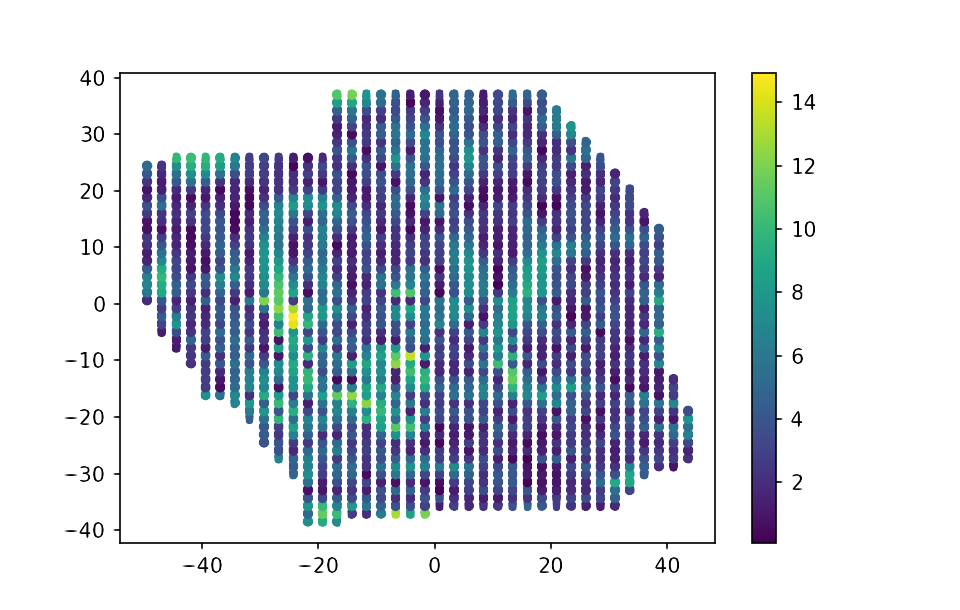
\includegraphics[width=0.75\textwidth]{./figure/figureSlope}
    \caption{The slope of each grid}
    \label{fig:figureSlope}
\end{figure}


    With each grid traversed by coordinates, we get a matrix describing all metrics in all grids -- see function~\eqref{eq:ama}.


    \subsubsection{Definitions}
        We first define the following concepts, each of which has no dimension:

        Define $M$ as the number of metrics.

        Define $N$ as the number of facilities.

        Define $Q$ as the type of facilities.

        Define $\alpha\left[\left( x , y \right), i , t \right]$ as the value of the $i^{th}$ metrics at position $\left(
x,y \right)$ and time $t$:

        \begin{equation}
            \label{eq:ama}
            \alpha=
            \begin{bmatrix}
                \begin{bmatrix}
                    \alpha_{(0,0),0}(t)\\
                    \vdots\\
                    \alpha_{(0,0),M-1}(t)\\
                \end{bmatrix}&
                \cdots&
                \begin{bmatrix}
                    \alpha_{(0,y_{max}-1),0}(t)\\
                    \vdots\\
                    \alpha_{(0,y_{max}-1),M-1}(t)\\
                \end{bmatrix}&\\
                \vdots&\ddots&\vdots\\
                \begin{bmatrix}
                    \alpha_{(x_{max}-1,0),0}(t)\\
                    \vdots\\
                    \alpha_{(x_{max}-1,0),M-1}(t)\\
                \end{bmatrix}&
                \cdots&
                \begin{bmatrix}
                    \alpha_{(x_{max}-1,y_{max}-1),0}(t)\\
                    \vdots\\
                    \alpha_{(x_{max}-1,y_{max}-1),M-1}(t)\\
                \end{bmatrix}
            \end{bmatrix}\Leftarrow
            \begin{bmatrix}
                x_{max}\\
                y_{max}\\
                M
            \end{bmatrix}
        \end{equation}

        which can also be written as:

        \begin{equation}
            \label{eq:amao}
            \alpha = \left [ \left [ \alpha_{\left ( x,y \right ),i }\left ( t \right )  \right ]_{i \in \left[ 0,M \right)}  \right ]_{x \in \left[ 0,x_{max} \right), y \in \left[ 0,y_{max} \right) }
        \end{equation}

        The upper matrix is a three-dimensional matrix with the maximum size of $x_{\max}$, $x_{\max}$, $M$.
        For each grid there are $M$ metrics in total, as there would be a $\begin{bmatrix} M \end{bmatrix}$
matrix to
describe the total $\alpha$ of the grade.

        For a clearer understanding, matrix $\alpha$ can be visualized as Figure~\ref{fig:figureVF}: at a certain moment
, the $x$ and $y$ axis indicate their position on the map, namely $\left(x, y\right)$ in the matrix.
        The three layers means the figure of grids and two of the $M$ metrics, which respectively are vegetation
coverage,grids and slope.

        \begin{figure}[H]
            \centering
            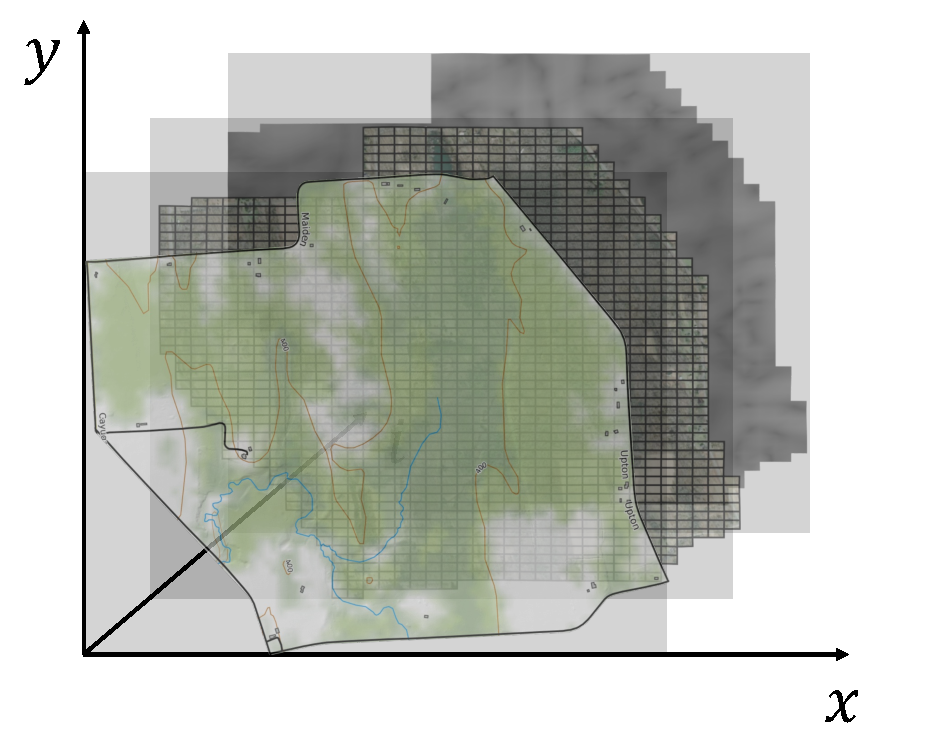
\includegraphics[width=0.5\textwidth]{./figure/figure1}
            \caption{Visulization of different indices conbining}
            \label{fig:figureVF}
        \end{figure}

        Define $U_{j, i}\left(\mathrm{pos}_k, \mathrm{pos}\right)$ as the impact of the $j^{th}$ kind facility in $\mathrm{
    pos}_k$ $\left(
x_k, y_k\right)$ on the value of $i^{th}$ metric in $\mathrm{pos}$ $\left( x, y \right)$.
        Here is the overall form of $U$:

        \begin{equation}
            \label{eq:bma}
            U=
            \begin{bmatrix}
                U_{0,0}(\cdot)&U_{0,1}(\cdot)&\cdots&U_{0,M-1}(\cdot)\\
                U_{1,0}(\cdot)&U_{1,1}(\cdot)&\cdots&U_{1,M-1}(\cdot)\\
                \vdots&\vdots&\ddots&\vdots\\
                U_{Q-1,0}(\cdot)&U_{Q-1,1}(\cdot)&\cdots&U_{Q-1,M-1}(\cdot)\\
            \end{bmatrix}
            =\left [ U_{j,i}\left ( \cdot \right )  \right ]_{j \in \left[0,Q\right),i \in \left[0,M\right)}
            \Leftarrow
            \begin{bmatrix}
                Q\\
                M
            \end{bmatrix}
        \end{equation}

        Define $V_{j, i}\left(\alpha \right)$ as the impact of the environment on the facility in its own grid where
facility type is $j$, metric is $i$ and the value of which is $\alpha$.
        The overall form of $V$ is:

        \begin{equation}
            \label{eq:cma}
            V=
            \begin{bmatrix}
                V_{0,0}(\cdot)&V_{0,1}(\cdot)&\cdots&V_{0,Q-1}(\cdot)\\
                V_{1,0}(\cdot)&V_{1,1}(\cdot)&\cdots&V_{1,Q-1}(\cdot)\\
                \vdots&\vdots&\ddots&\vdots\\
                V_{M-1,0}(\cdot)&V_{M-1,1}(\cdot)&\cdots&V_{M-1,Q-1}(\cdot)\\
            \end{bmatrix}
            =\left [ V_{i,j}\left ( \cdot \right )  \right ]_{i \in \left[0,M\right),j \in \left[0,Q\right)}
            \Leftarrow
            \begin{bmatrix}
                M\\
                Q
            \end{bmatrix}
        \end{equation}

        Define $W$ as the weight of each metric:

        \begin{equation}
            \label{eq:dma}
            W=
            \begin{bmatrix}
                w_0\\
                w_1\\
                \vdots\\
                w_{M-1}
            \end{bmatrix}\Leftarrow
            \begin{bmatrix}
                M\\
            \end{bmatrix}
        \end{equation}

        Define $A_k\left(t \right)$ as the activity of the $k^{th}$ facility at moment $t$, while the information of
the $
k^{th}$ facility as well contains its position $\left( x_k, y_k \right)$ and its type $\text{type}_k$.

        The overall matrix form of $A\left(t \right)$ is:

        \begin{equation}
            \label{eq:ema}
            A(t)=
            \begin{bmatrix}
                A_0(t)\\
                A_1(t)\\
                \vdots\\
                A_{N-1}(t)
            \end{bmatrix}\Leftarrow
            \begin{bmatrix}
                N\\
            \end{bmatrix}
        \end{equation}

        whose calculation formula is:

        \begin{equation}
            \label{eq:emc}
            A(t)=
            \begin{bmatrix}
                \frac{
                    \begin{bmatrix}
                        V_{i,\mathrm{type}_k}(a_{\mathrm{pos}_k,i}(t))
                    \end{bmatrix}_{i\in [0,M)}\times W^T}{\sum W}
            \end{bmatrix}_{k\in [0,N)}
        \end{equation}

        Define $S$ as the function to describe the relation between the profit and time for every kind of facility, and can present as a matrix:

        \begin{equation}
            \label{eq:fma}
            S=
            \begin{bmatrix}
                S_0(t)\\
                S_1(t)\\
                \vdots\\
                S_{Q-1}(t)
            \end{bmatrix}
        \end{equation}

        Define $h_c \left( t \right)$ as the function describing the relation between the conversion rate and time,
where $c = 1$ or $2$; when $c = 1$, $h_c \left( t \right)$ stands for long-term function and when $c = 2$, $h_c \left( t
\right)$ stands for short-term one.
        For instance, we can design the $h-t$ function like the sigmoid function $\sigma$ in Figure~\ref{fig:figureExample}
        below.

        \begin{figure}[H]
            \centering
            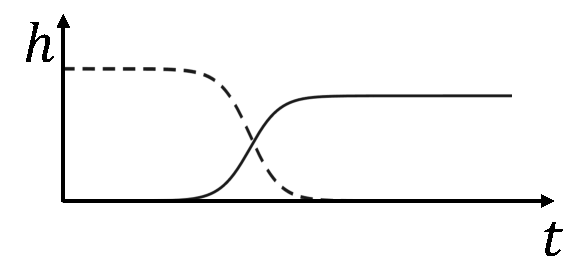
\includegraphics[width=0.3\textwidth]{./figure/figureSigmoid}
            \caption{An example for the $h-t$ function ($h_1-t$ is the solid line; $h_2-t$ is the dotted line)}
            \label{fig:figureExample}
        \end{figure}

        As we see, the value of $h_1\left( t \right)$ in the beginning is low, while that of the $h_2\left( t \right)$ is comparatively high.
        After crossing the defined boundary of \lq\lq short-term \rq\rq and \lq\lq long-term \rq\rq, the size relation of those two value interchange.
        The figure of $h_c \left( t \right)$ can well describe the trend of long-term and short-term profit.

        Define $P\left( r, t_{total}, \alpha_0, W \right)$ as the coefficient of profit;
        where $r$ is the weight of long-term profit and correspondingly $\left( 1 - r \right)$ is the
weight of short-term profit,
        $t_{total}$ is the total time the decision-maker considers and $\alpha_0 $ is the value of $\alpha$ when $t
= 0$.

    \subsubsection{Differential and Simulation}

In order to quantify the mutual influence between facilities and the environment, we take differential equations into
consideration.
Since the changing rate of $\alpha$ is dependent on the activity of facilities, their influence, and time, we decided to
use differential equations to describe and quantify the relations.
The equations are:

        \begin{equation}
            \frac{\mathrm{d} \alpha_{\mathrm{pos}, i}\left ( t \right ) }{\mathrm{d} t} = A\left ( t \right )^T \times \left [ U_{\mathrm{type}_k, i}\left ( \mathrm{pos}_k, \mathrm{pos} \right ) \right ]_{k \in \left[ 0,N \right)}
            \label{eq:fuck}
        \end{equation}

        \begin{equation}
            \label{eq:aaa}
            A(t)=
            \begin{bmatrix}
                \frac{
                    \begin{bmatrix}
                        V_{i,\mathrm{type}_k}(a_{\mathrm{pos}_k,i}(t))
                    \end{bmatrix}_{i\in [0,M)}\times W^T}{\sum W}
            \end{bmatrix}_{k\in [0,N)}
        \end{equation}

        \begin{equation}
            \alpha \left( 0 \right) = \alpha_0
            \label{eq:asdf}
        \end{equation}



        For the differential equation, the right part of it conveys the idea mentioned above.
        The result of matrix of the overall activity cross matrix of the overall mutual influence on position $\left(x,y
\right)$ reflects the total absolute impact on  $\left(x,y\right)$ \rq{s} $\alpha_{\mathrm{pos}, i}$.
\eqref{eq:aaa} means that the activity of a facility equals to the sum of all products of the impact times
corresponding weight and divide by the sum of all weights.
Function \eqref{eq:asdf} stands for the initialization of $\alpha$


    \subsubsection{Integral and Profit Calculating}
        In order to quantify the profit, we have to integrate all the profit-related coefficients and functions
        mentioned above.
        We have already defined a function that consists of all these things: $P\left( r, t_{total}, \alpha_0, W
\right)$; then we analyze the relation between the vital variables $t$ and $t_{total}$, and sort out the integral
equations:

        For long-term profit, there is:

        \begin{equation}
            \label{eq:ltp}
            P_{long}\left(r_0,T,\alpha_0,W\right) = \int_0^T r_0 h_1\left(t\right){A
            \left(t\right)}^T\times
            \begin{bmatrix}
                S_{\mathrm{type}_k}\left(t\right)
            \end{bmatrix}_{k\in \left[0,N\right)}
            \mathrm{d}t
        \end{equation}

        For short-term profit, there is:

        \begin{equation}
            \label{eq:stp}
            P_{short}\left(1-r_0,T,\alpha_0,W\right) = \int_0^T \left( 1-r_0 \right)h_2\left(t\right){A
            \left(t\right)}^T\times
            \begin{bmatrix}
                S_{\mathrm{type}_k}\left(t\right)
            \end{bmatrix}_{k\in \left[0,N\right)}
            \mathrm{d}t
        \end{equation}

        where the left parts of the upper equations are the total of coefficient of profit and the right parts are long-term profit or short-term profit.
        These two profit data are calculated by multiplying activity, the profit and the conversion
rate, which accords to the left of the equation and proves the rationality of the integral relation.

        Obviously:
        \begin{equation}
            \label{eq:tp}
            P_{total} = P_{long} + P_{short}
        \end{equation}

        Overall, consider equation~\eqref{eq:ltp}~\eqref{eq:stp}~\eqref{eq:tp}:

        \begin{equation}
            \label{eq:itp}
            P\left(r_0,T,\alpha_0,W\right)=\int_0^T\left(r_0 h_1\left(t\right)+\left(1-r_0\right)h_2
            \left(t\right)\right){A
            \left(t\right)}^T\times
            \begin{bmatrix}
                S_{\mathrm{type}_k}\left(t\right)
            \end{bmatrix}_{k\in \left[0,N\right)}
            \mathrm{d}t
        \end{equation}

    \subsection{Sub-model I: Diffusion Equation}
        By taking degradation and absorption out of consideration and viewing the diffusion of the polluted chemical
        as an one -dimensional dynamic system, we can describe the diffusion of the pollution in the soil with the time fractional diffusion equation:

        \begin{equation}
            \label{eq:tfd}
            D\cdot \frac{\partial^2 C\left(x, t \right)}{\partial x^2} - \frac{\partial C\left( x, t
            \right)}{\partial t} = 0
        \end{equation}

        The equation is a second order partial differential equation, so we need to find two boundary conditions:
        Semi-infinite boundary and Cauchy boundary.
        The Semi-infinite boundary refers that the concentration gradient of a place that is infinitely far from the source
        is $0$, which is suitable when the weight of diffusion in the whole spreading process is big.

        \begin{equation}
            \label{eq:sib}
            \frac{\partial C\left(x, t\right)}{\partial x} = 0,\ x = \infty
        \end{equation}

        The Cauchy boundary is a mixture of several kind of condition, which can be written in the form of:

        \begin{equation}
            \label{eq:cb}
            \lambda \frac{\partial C\left(x, t\right)}{\partial x} + \mu C\left(x, t\right) = 0,\ x = H
        \end{equation}

        $\lambda$ and $\mu$ are both the constant of the boundary condition, and $\frac{\mu}{\lambda}$ is the boundary parameter.

        Then it is able can solve this equation by using these two boundary conditions.
        The two boundary conditions is involved in integrating of the equation, as well as the original condition.

        The solution of the equation is:

        \begin{equation}
            \label{eq:se}
            C\left(x, t\right) = \frac{\frac{Q}{K_d} \exp{\frac{-x^2}{4D\rho t}}}{\left(4\pi D\rho t\right)^{\frac{3}{2}}}
        \end{equation}

        In the equation, $D$ is the average diffusion coefficient of all the polluted chemicals, $Q$ is the total amount of the chemicals that is polluted from the beginning to the end of the investigation period.
        $\rho$ is the bulk density of the soil, which measures the mass density and porosity of the soil, both of which are related to the diffusion.
        $K_d$ is the soil-water partition coefficient, $t$ for time, and $x$ is the distance between the source and the observe spot.

        However, in order to better use this sub-model to meet with our overall model, the variable $t$ should be
        eliminated because the diffusion process spans too short on timescale in comparison with our boundaries for
short-term and long-term profit (which are respectively $1$ year and $10$ years).
        As we only consider a static state of pollutants being diffused, the impact of the pollution would stay still
on timescale and is only related to the distance between the source of pollution and the detecting point.

The result is:

        \begin{equation}
            \label{eq:nte}
            C\left(x\right) = \frac{Q}{K_d \cdot 4\pi D\rho x}
        \end{equation}

    \subsection{Sub-model II: Impact Function of Environment to Facility}
    According to the assumptions, we regard the possibility distribution of geological metrics as normal distribution.
    By collecting data, we discovered that there is always a proper range of each metric $\left( \alpha_{min}, \alpha_{
    max} \right)$, where the most suitable value of the metric $\alpha_{suit}$ also exists in the range.
    The value of $V$ also has its range as it has positive relation with $\alpha$.
    Thus, there should be:

    \begin{equation}
        \label{eq:vcd}
        V_{i,j}\left( \alpha \right) \sim N\left( \mu, \sigma^2 \right)
    \end{equation}

    $\mu = \frac{\alpha_{max} + \alpha_{min}}{2}$ is the arithmetic mean and $\sigma$ is the standard deviation.

    Then, we define $q\left( l, r, \mu, \sigma \right)$ as the shadow area in Figure~\ref{fig:figureArea}.

    \begin{figure}[H]
        \centering
        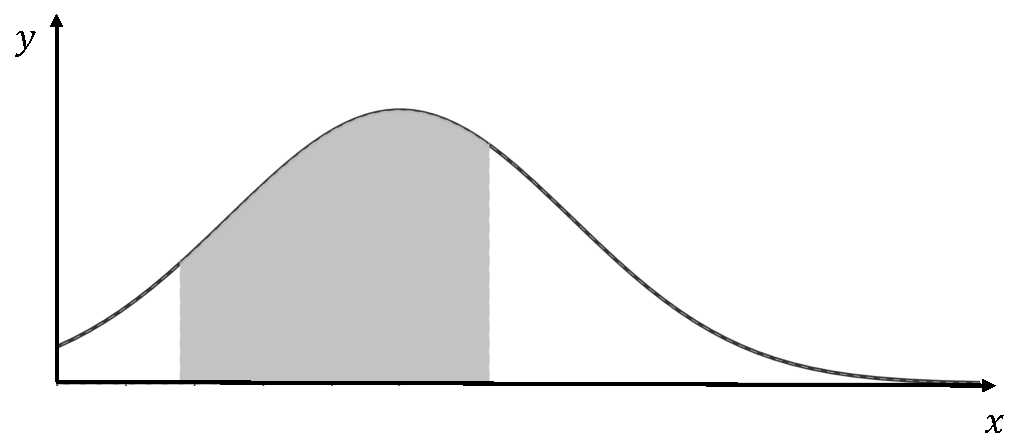
\includegraphics[width=0.8\textwidth]{./figure/figureERFshade}
        \caption{The Actual Meaning of Function $q$}
        \label{fig:figureArea}
    \end{figure}

    where $l$ and $r$ respectively refers to the minimum and the maximum of the metric $i$ in a specific position.
    It is proved that the calculation formula of $q$ is:
    \begin{equation}
        \label{eq:erf}
        q\left( l, r, \mu, \sigma \right) = \frac{1}{2} \text{erf} \left( \frac{x-\mu}{\sqrt{2}\sigma } \right)\bigg|_{l}^{r}
    \end{equation}

    In order to make sure the $\sigma$ of the normal distribution is reasonable, we need to determine the threshold
of the distribution, which can be present as the following form.

    \begin{equation}
        \label{eq:ts}
        \frac{q\left( l_{{i}_{suit}}, r_{{i}_{suit}}, \mu_i, \sigma \right)}{q\left( \alpha_{{i}_{min}}, \alpha_{{i}_{max}}, \mu_i, \sigma \right)}
        = Ts
    \end{equation}

    We artificially determine a reasonable threshold $Ts$ to be 50\%.
    In the equation, $l$, $r$, $\alpha_{min}$, $\alpha_{max}$, $\mu$ and $Ts$ are all known constants, hence we can
use the iterative method to solve the standard deviation.
    The solution of $\sigma$ helps us to quantify and add up the value of different metric and calculate the overall $V$.

    The equation of $V$ after normalization is:

    \begin{equation}
        \label{eq:nv}
        V_{i, j}\left( \alpha \right) = \frac{1}{\sqrt{2\pi}q\left( \alpha_{{i}_{min}}, \alpha_{{i}_{max}}, \mu_i, \sigma \right)\sigma}\exp \left( -\frac{\left( x-\mu \right)^2}{2\sigma^2} \right)
    \end{equation}

\end{document}